%%%%%%%%%%%%%%%%%%%%%%%%%%%%%%%%%%%%%%%%%%%%%%%%%%%%%%%%%%%%%%%%%%%%
%% I, the copyright holder of this work, release this work into the
%% public domain. This applies worldwide. In some countries this may
%% not be legally possible; if so: I grant anyone the right to use
%% this work for any purpose, without any conditions, unless such
%% conditions are required by law.
%%%%%%%%%%%%%%%%%%%%%%%%%%%%%%%%%%%%%%%%%%%%%%%%%%%%%%%%%%%%%%%%%%%%

\documentclass[
  digital, %% This option enables the default options for the
           %% digital version of a document. Replace with `printed`
           %% to enable the default options for the printed version
           %% of a document.
  table,   %% Causes the coloring of tables. Replace with `notable`
           %% to restore plain tables.
  lof,     %% Prints the List of Figures. Replace with `nolof` to
           %% hide the List of Figures.
  lot,     %% Prints the List of Tables. Replace with `nolot` to
           %% hide the List of Tables.
  %% More options are listed in the user guide at
  %% <http://mirrors.ctan.org/macros/latex/contrib/fithesis/guide/mu/sci.pdf>.
]{fithesis3}
%% The following section sets up the locales used in the thesis.
\usepackage[resetfonts]{cmap} %% We need to load the T2A font encoding
\usepackage[T1,T2A]{fontenc}  %% to use the Cyrillic fonts with Russian texts.
\usepackage[
  main=czech, %% By using `czech` or `slovak` as the main locale
                %% instead of `english`, you can typeset the thesis
                %% in either Czech or Slovak, respectively.
  german, russian, czech, slovak %% The additional keys allow
]{babel}        %% foreign texts to be typeset as follows:
%%
%%   \begin{otherlanguage}{german}  ... \end{otherlanguage}
%%   \begin{otherlanguage}{russian} ... \end{otherlanguage}
%%   \begin{otherlanguage}{czech}   ... \end{otherlanguage}
%%   \begin{otherlanguage}{slovak}  ... \end{otherlanguage}
%%
%% For non-Latin scripts, it may be necessary to load additional
%% fonts:
\usepackage{paratype}
\def\textrussian#1{{\usefont{T2A}{PTSerif-TLF}{m}{rm}#1}}
%%
%% The following section sets up the metadata of the thesis.
\thesissetup{
    date          = \the\year/\the\month/\the\day,
    university    = mu,
    faculty       = sci,
    department    = Ústav chemie,
    departmentEn  = Department of Mathematics and
                    Statistics,
    programme     = Chemie,
    programmeEn   = Chemistry,
    field         = Chemie,
    fieldEn       = Chemistry,
    type          = bc,
    author        = Petra Hrozková,
    gender        = f,
    advisor       = doc. Mgr. M. Munzarová Dr. rer. nat ,
    title         = Studium vlivu koordinačního prostředí atomů Si a P na tvorbu SiO6 center metodami EHT a DFT,
    TeXtitle      = Studium vlivu koordinačního prostředí atomů Si a P na tvorbu SiO6 center metodami EHT a~DFT,
    titleEn       = A combined EHT/DFT study of Si and P coordination environment influence on the creation of SiO6 centers,
    TeXtitleEn    = The Principles of the Typesetting of
                    Mathematics in \TeX: the Program,
    keywords      = {klíčové slovo 1, klíčové slovo 2, ...},
    TeXkeywords   = {klíčové slovo 1, klíčové slovo 2, \ldots},
    keywordsEn    = {keyword1, keyword2, ...},
    TeXkeywordsEn = {keyword1, keyword2, \ldots},
}
\thesislong{abstract}{
    This is the abstract of my thesis, which can

    span multiple paragraphs.
}
\thesislong{abstractEn}{
    This is the English abstract of my thesis, which can

    span multiple paragraphs.
}
\thesislong{thanks}{
    This is the acknowledgement for my thesis, which can

    span multiple paragraphs.
}
%% The following section sets up the bibliography.
\usepackage{csquotes}
\usepackage[              %% When typesetting the bibliography, the
  backend=biber,          %% `numeric` style will be used for the
  style=numeric,          %% entries and the `numeric-comp` style
  citestyle=numeric-comp, %% for the references to the entries. The
  sorting=none,           %% entries will be sorted in cite order.
  sortlocale=auto         %% For more unformation about the available
]{biblatex}               %% `style`s and `citestyles`, see:
%% <http://mirrors.ctan.org/macros/latex/contrib/biblatex/doc/biblatex.pdf>.
\addbibresource{example.bib} %% The bibliograpic database within
                          %% the file `example.bib` will be used.
\usepackage{makeidx}      %% The `makeidx` package contains
\makeindex                %% helper commands for index typesetting.
%% These additional packages are used within the document:
\usepackage{paralist}
\usepackage{amsmath}
\usepackage{amsthm}
\usepackage{amsfonts}
\usepackage{url}
\usepackage{menukeys}
\begin{document}
\chapter{Úvod}

\begin{otherlanguage}{czech}
Motivace experimentální prací Mgr. Aleše Stýskalíka PhD. 



 \begin{figure}[h!]
\caption{Silikofosfátová síť. \cite{Styskalik2015thesis} }
  \center
  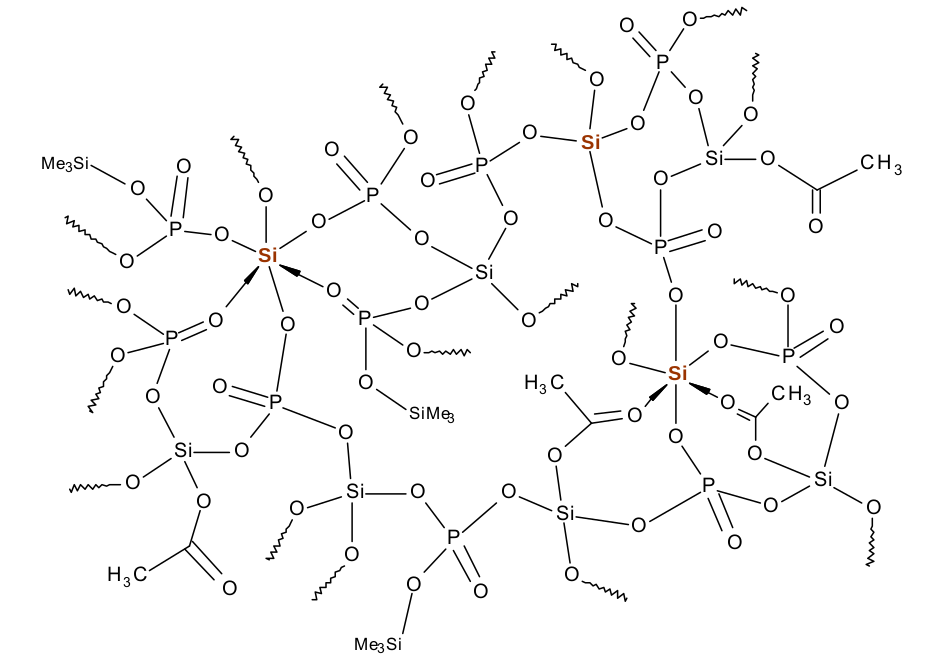
\includegraphics[width=15cm]{si_polymer_cely.png}
  \label{si_polymer_cely}
  \end{figure}

\begin{figure}[h!]
\caption{Prostředí kolem Si. \cite{Styskalik2015thesis} }
  \center
  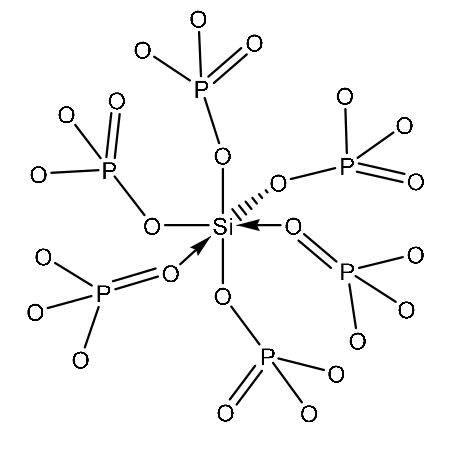
\includegraphics[width=10cm]{si_koordinovane_6_P.png}
  \label{si_koordinovane_6_P}
  \end{figure}
  
  \begin{figure}[h!]
\caption{Prostředí kolem Si. \cite{Styskalik2015thesis} }
  \center
  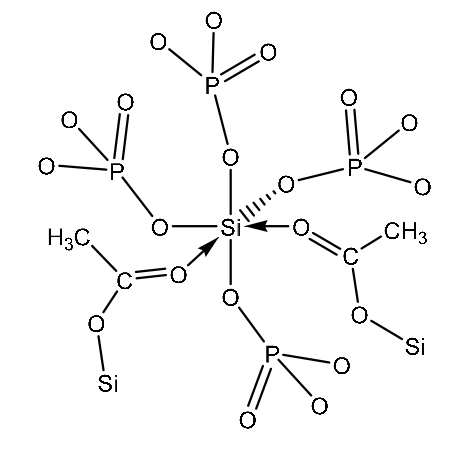
\includegraphics[width=10cm]{si_koordinovany_6_C.png}
  \label{si_koordinovany_6_C}
  \end{figure}
\end{otherlanguage}



\chapter{Teoretická část}
Znalosti o chemické vazbě jsou klíčovou schopností pro každý experiment. S touto znalostí je možno předpokládat průběh experimentu a částečně i strukturu. S chemickou vazbou jsou neoddělitelně spojeny atomy. Počátky atomové teorie datujeme v letech 430-310 př.n.l v Řecku. Autorem je Démokritos, který předpokládal, že hmota je stvořena z malých, dále nedělitelných částí. Počátky molekulové struktury jsou v 18.století, kdy John Dalton použil atomovou teorii k vysvětlení chemických reakcí. Zároveň formuloval zákon stálých poměr slučovacích a zákon stálých poměrů násobných. V roce 1852 se objevuje myšlenka valence elektronů, která ovšem není kompletní do objevení elektronu 1897 Thomsonem. \\
Lewis jako první nahlížel na chemickou vazbu jako párování elektronů. \cite{Munzarova1996thesis} \\
Asi největší přínos do teorie chemické vazby měl zrod kvantové mechaniky. Zpočátku se jednalo pouze o popis elektronů v atomu vodíku. S pokrokem v matematice, výpočetní technice a fyzice se z toho časem široké spektrum metod, které více či méně dobře popisují chemickou vazbu.\\
První kvantověmechanický popis zavedl Heitler a London ve své teorii valenčních vazeb (Valence Bond Theory, VB). Teorie navazuje na myšlenku sdílení elektronových páru od Lewise. Ústřední myšlenkou jsou vazebné orbitaly, kdy největší elektronová hustota je na spojnici dvou sousedních atomů. Spojením dvou atomových orbitalů vzniká vazebný orbital. Tomuto popisu se vymyká například uhlík, proto byl vymyšlen koncept hybridizace. Hlavní myšlenkou je, že dojde k spojení orbitalů, které jsou si blízké v energii. Vzniknou tak rovnocenné hybridní orbitaly. \cite{Munzarova1996thesis} \\
Nedostatky VB teorie se pokusila řešit teorie molekulových orbitalů, MO. Ta nahlíží na molekulu podobně jako na atom, vytváří koncept molekulových orbitalů. Elektronová hustota je delokalizována přes všechny atomy.\cite{Munzarova1996thesis} \\
\section{Vlnová funkce a Schrödingerova rovnice}
Vlastnosti chemických molekul určují především elektrony. Ve 20. století již bylo známo, že elektrony se svým chováním vymykají představám klasické mechaniky. Na počátku 20. století bylo popsáno chování černého tělesa, fotoeletkrického jevu a představám, že svět není spojitý. Myšlenka, že svět je tvořen z diskrétních částí vedla k vzniku kvantové mechaniky. U jejího zrodu stál třeba W. Heisenberg, E. Schrödinger a P. A. M. Dirac. V běžné mechanice je systém možné přesně popsat polohou a hybnosti, díky těmto veličinám lze předvídat i pohyb budoucí. V kvantové mechanice je základem Schrödingerova rovnice \ref{SCH_rce_kratka}, diferenciální rovnice druhého řádu, která v sobě obsahuje veškerou informaci o systému.\cite{polak2000obecna}
\begin{equation}
\widehat{H} \Psi = E \Psi
\label{SCH_rce_kratka}
\end{equation}
$\widehat{H}$ je Hamiltonián, operátor, který reprezentuje energii systému. $E$ je energie, vlastní hodnota Hamiltoniánu. $\Psi$ je vlnová funkce, která v sobě ukrývá celou informaci o systému. Hamiltonián se skládá ze dvou částí, operátoru kinetické a potenciální energie.
\begin{equation}
\widehat{H} = \widehat{T} + \widehat{V}
\end{equation}
$\widehat{T}$ reprezentuje kinetickou enregii, $\widehat{V}$ je potenciální energie.
Výraz pro kinetickou energii $\widehat{T}$, který v sobě zahrnuje všechny částice systému. 
\begin{equation}
\widehat{T} = - \frac{h^2}{8 \pi ^2} \sum \frac{1}{m_i} \left( \frac{\delta^2}{\delta x_i^2} +\frac{\delta^2}{\delta y_i^2} +\frac{\delta^2}{\delta z_i^2} \right)
\end{equation}
$\hbar$  je Planckova konstanta\footnote{6, 626  $\cdot 10^{-34} ~ J \cdot s$}, $m_i$ je hmotnost i-té částice. Výraz pro potenciální energii $\widehat{V}$ je coulombovská interakce mezi částicemi.
\begin{equation}
\widehat{V} = \sum_{i<j}\sum \left( \frac{e_i e_j}{r_{i,j}}\right)
\end{equation}
 Pro chemické účely postačí stacionární Schrodingerova rovnice, která v sobě nezahrnuje čas.
\begin{equation}
-\frac{\hbar^2}{2m_i} \frac{d^2 \psi}{d\vec{r} ^2} + V(\vec{r}) \psi = E \psi
\label{schrodingerova_rovnice}
\end{equation}
Vlnovou funkci lze získat řešením Schrödingerovy rovnice \ref{schrodingerova_rovnice}. Přesto exaktní řešení existuje pouze pro atom vodíku a další exotické atomy, které mají jeden elektron a jeden proton. Základním přístupem je separace pohybu elektronů od pohybu jader kvůli velkým rozdílům v hmotnosti těchto částic. Rozložení elektronů je tak závislé pouze na poloze elektronu, nikoli na rychlosti. Separace problému na dva samostatně řešitelné přístupy se nazývá Born-Oppenheimerova aproximace nebo adiabatická aproximace. \cite{warren1986ab}
Řešením rovnice \ref{schrodingerova_rovnice} pro atom vodíku získáme energii a orbitaly, jednoelektronovou funkci. Orbital je matematický prostor, kde se elektron vyskytuje s nejvyšší pravděpodobností. Fyzikální význam má pouze $|\Psi|^{2}$. V atomech se nachází atomové orbitaly. \\
Přidáním elektronů do vícelektronového atomu se v rovnici objeví vzájemné působení elektronů a rovnice se stává analyticky neřešitelnou. Zde přichází na řadu numerické a přibližné metody. První způsob řešení elektronů v atomech je model neinteragujících elektronů, které se pohybují nezávisle na sobě. Tato aproximace pochopitelně nemá pro chemii význam, lze ji použít v ojedinělých případech pro ionty. Pro popis atomů s více elektrony lze použít již zmíněné atomové orbitaly. Příslušnou vlnovou funkci pro atom s více elektrony lze zapsat součin jednoelektronových funkcí. Vyjádření víceelektronové vlnové funkce jako součin jednoelektronových funkcí navrhl Hartree. Základ jeho metody je přístup, že elektron interaguje s průměrným polem ostatních elektronů. V základu je navrhnuta hrubá vlnová funkce, která je pomocí variačního počtu vylepšována, až je nalezena vlnová funkce, která poskytuje nejnižší energii.
\begin{equation}
\psi_{AO} = 1s(1)
\end{equation}
\begin{equation}
\psi_{MO} = 1s(1) \cdot 2s(1)
\end{equation} 
Všechny orbitaly musí být vzájemně orthogonální a normalizované.
\begin{equation}
S_{ii} = \int \psi_i * \psi_i dx dy dz = 1 ~ \bigwedge ~ S_{ij} = \int \psi_i * \psi_j dx dy dz = 0
\end{equation}
V tomto přístupu jsou ovšem elektrony číslovány a není dodržena antisymetrii vlnové funkce (Pauliho princip). \cite{warren1986ab}
\begin{equation}
\Psi (1,2) = - \Psi (2,1)
\label{Paulliho_princip}
\end{equation}
 Každá jednoelektronová funkce má prostorou a spinovou část, tzv. spinoorbital. Pro mnohaelektronové atomy už je nutno spin vzít v úvahu. Antisymetrii a spin lze do výsledné vlnové funkce zahrnout s pomocí Slaterova determinantu, SD, který má obecný tvar \ref{Slateruv_determinant}. SD zaručuje antisymetrii vlnové funkce vůči výměně polohových nebo spinových souřadnic. $\psi_i$ je jednoelektronová vlnová funkce, $s_j$ jsou elektrony, $\sqrt{N!}$ je normalizační faktor.
\begin{equation}
\psi =  \frac{1}{\sqrt{N!}}\begin{vmatrix}
\psi_1(1)\alpha(1) & \psi_1(1) \beta (1) & \psi_2(1)\alpha(1) & \dots & \psi_{n/2}(1)\beta(1) \\
\psi_1(2)\alpha(2) & \psi_1(2) \beta (2) & \psi_2(2)\alpha(2) & \dots & \psi_{n/2}(2)\beta(2) \\
\vdots             & \vdots              & \vdots             & \ddots & \vdots \\
\psi_1(n)\alpha(n) & \psi_1(n) \beta (n) & \psi_2(n)\alpha(n) & \dots & \psi_{n/2}(n)\beta(n) 
\end{vmatrix}
\label{Slateruv_determinant}
\end{equation}
Jednoelektronové funkce, ze kterých je tvořena mnohaelektronová funkce, tvoří prostor úplných bazí. Základní typem jsou Slaterovy báze a gaussovské báze. (více v kapitole \ref{kapitola_baze})




\subsection{Hypervalence}
\subsection{Teorie molekulových orbitalů}

\section{Metody kvantové chemie}
Metody výpočetní chemie lze ve stručnosti shrnutou na \textit{Ab inito} metody, semi-empirické metody a DFT metody. \textit{Ab inito} metody řeší Schröfingerovu rovnici bez použití parametrů z experimentálních dat.  Vzájemnou souvislost a podobnost metody vystihuje schéma na obrázku \ref{schema_QM}.
 \begin{figure}[h]
\caption{Schéma post-Hartree-Fockových teorií, $n^m$ je škálování vzhledem k velikosti systémy \cite{pdf_obrazek}. }
  \center
  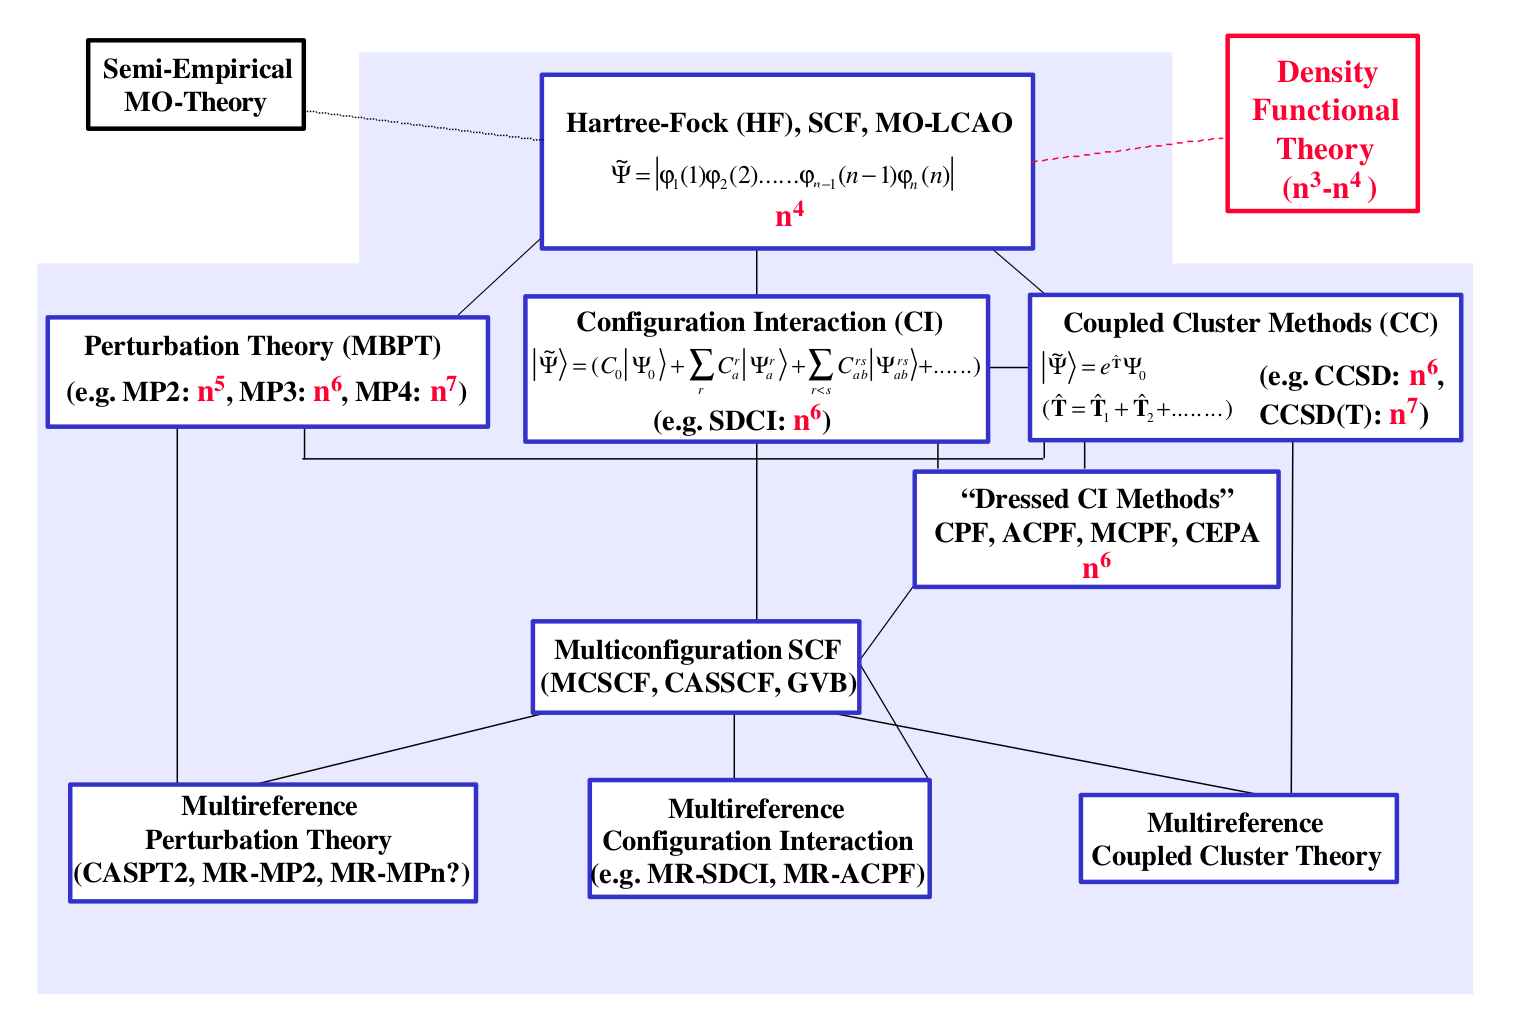
\includegraphics[width=12cm]{schema_QM.png}
  \label{schema_QM}
  \end{figure}
  Metody QM vychází z řešení stacionární Schrödingerovy rovnice \ref{schrodingerova_rovnice}. Semiempirické metody řeší Schrödingerovu rovnici pouze částečně, některé parametry jsou dodány z experimentů. \\
     Základní aproximací je Born-Oppenheimerova aproximace a zapsání vlnové funkce jako Slaterův determinant pomocí atomových orbitalů. Z tohoto základu vznikla Hartree, která navíc uvažuje elektron v průměrném poli zbylých elektronů. Zde pomocí variačního přístupu hledá nejvhodnější energii. Antysymetrii vlnové funkce zajistí SD a Fockovy rovnice, proto Hartee-Fockova metoda. Samotný HF přístup v sobě neobsahuje korelaci pohybu elektronů. Tento faktor je tam možno vložit dodatečně pomocí tradičních \textit{ab inito} metod Many-Body Pertrubation  theory (MBPT), konfigurační interakcce (configuration interaction, CI) nebo spřažené klastry( coupled cluster methods, CC). Śkálování těchto metod je uvedeno na obrázku \ref{schema_QM}. Tyto metody jsou přesné, ale výpočetně velice náročné proto nejsou vhodné pro příliš velké systémy. Řešením je použití teorie funkcionálu hustoty (The Density Functional theory, DFT) nebo Rozšířenou Hückelovu metodu (The Extenden Hückle theory, EHT).

\section{Rozšířená Hückelova metoda}
EHT se řadí mezi semiemprické metody, které  pro výpočet energie používají klasický \textit{ab inito} přístup, pouze jsou některé parametry vzaty z experimentu. Tím se snižuje výpočetní náročnost. Přes její jednoduchost dává dobré kvalitativní výsledky především v oblasti molekulových orbitalů. EHT navazuje na Hückelův přístup, který platil pro konjugované systémy. EHT může být použita i pro systémy se $\sigma$ vazbami. Na rozvoji teorie se podílel Roald Hoffman. \cite{lowe2011quantum} \\
Základem metody je sekulární rovnice, která je známá již z metody MO-LCAO. (viz. sekulární rovnice v metody MO-LCAO). EHT poskytuje jednoduché řešení členu $H_{ij}$ pomocí vzorce \ref{EHT_vypocet_H} a empirických parametrů. $S_{ij}$ je překryvový integrál, $E$ je hlednanní energie.
\begin{equation}
E = \begin{vmatrix}
H_{11} - E S_{11} & H_{12} - E S_{12} & \dots & H_{1j} - E S_{1j} \\
H_{21} - E S_{21} & H_{12} - E S_{22} & \dots & H_{1j} - E S_{2j} \\
\vdots & \vdots &  \ddots & \vdots  \\
H_{i1} - E S_{i1} & H_{i2} - E S_{i2} & \dots & H_{ij} - E S_{ij} \\
\end{vmatrix}
\end{equation}


\begin{equation}
H_{ij} = K S_{ij} \left( \frac{H_{ii} + H_{jj}}{2} \right)
\label{EHT_vypocet_H}
\end{equation}
kde $K$ si parametr, jehož hodnota byla R. Hoffmannnem stanoevna na 1,75. 

\section{Metoda funkcionálu hustoty}
DFT metody jsou založeny na vztahu mezi elektronovou hustotou a celkovou energii systému, teorie funkcionální \footnote{Funkcionál je operátor, který zobrazuje z prostoru funkcí do množiny obecně komplexních čísel} hustoty. Elektronová hustota $\varrho(\pmb{r})$ je pravděpodobnosti, že v nějakém bodě prostoru nalezneme nějaký elektron.  Výhodou tohoto přístupu je, že elektronová hustota je funkcí pouze tří prostorových souřadnic. Tento výpočetní model byl objeven už v roce 1920, pro chemii začal mít význam až v 60. letech 20. století. Výpočetně podobně náročná jako HF, ale přesnější, obsahují korelační energii. \\

V roce 1964 uveřejnili Koch a Hohenberg dva teorémy, které ukázaly, že energie základního stavu  a další vlastnosti jsou jednoznačně určeny elektronovou hustotou. Energie je funkcionál elektronové hustoty .
\cite{lechamolecularmodeling}
\subsection{Principy}
\subsubsection{První Hohenberg- Kohn teorém}
Pro libovolný systém interagujících elektronů je externí potenciál v ext jednoznačně
určen elektronovou hustotou (až na konstantu)
\subsubsection{Druhý Hohenberg-Kohn teorém}
Druhý teorém je postaven na variačním principu.
\cite{koch2000chemist} 
Předpokládejme, že danému externímu potenciálu V ext přísluší elektronová hustota
$\varrho_0$. Pak pro jakoukoli jinou elektronovou hustotu $\varrho$
0 bude platit
\begin{equation}
E [\varrho_0] < E[\varrho ']
\end{equation}
Druhý teorém je přístup, jakým způsobem hledat správný funkcionál.
\subsubsection{Kohn-Shamovy rovnice}
Při hledání vhodného funkcionálu je zásadní problém zahrnout kinetickou energii elektronů, klasickou coulombickou interakci mezi elektrony a dále korelační a výměnné efekty. Kinetickou energii lze započítat jako součet kinetické energie jednotlivých elektronů popsaných jednoelektronovou funkcí. Součet $E_{kin}$ pro jednotlivé elektrony poskytnou celkovou kinetickou energii \ref{kineticka_energie_jednoelektronova}. \cite{dftshrnutivysledky}
\begin{equation}
E_{kin} = -\frac{1}{2} \sum_{i=1} ^{N} \int \varphi \Delta_i \varphi d \vec{r}_i
\label{kineticka_energie_jednoelektronova}
\end{equation}
\subsection{DFT v praxi}
Výběr vhodného funkcionálu je nelehký úkol. Funkcionály mohou být obecně rozděleny na tři kategorie. Aproximace lokální hustoty (Local Density Approximation, LDA), metoda zoběcněného gradientu (Generalized Gradient Approximation, GGA) a poté hybridní funkcionály. \cite{dftshrnutivysledky}
\subsubsection{Aproximacce lokální hustoty}
LDA funkcionály vychází z modelu homogenního elektronového plynu, kdy máme v celém systému konstantní elektronovou hustotu.\cite{dftshrnutivysledky} V základu se jedná o \textit{ab inito} přístup, přesto má pro chemii využití pouze pro valenční elektrony. Často totiž v molekulách není pravidelná distribuce elektronové hustoty. Prostor lze rozdělit na jednotky objemu a elektronovou hustotu sčítat přes objem podle rovnice.
\begin{equation}
E_{XC}^{LDA} = \int \varrho (\vec{r} \epsilon_{XC} (\varrho (\vec{R})) d \vec{r}
\label{LDA_vyraz_pro_obecnou_energii}
\end{equation}
Tvar $\epsilon_{XC}(\varrho (\vec{r}))$je výměnně-korelační energie pro jeden elektron, která může být rozdělena na výměnnou a korelační část. 
\begin{equation}
\epsilon_{XC}(\varrho (\vec{r})) = \epsilon_x (\varrho) + \epsilon_c (\varrho)
\label{LDA_tvar_vymene_korelacni_energie}
\end{equation}
Výměnný člen lze zapsat analyticky, známy pod názvem Slaterův výměnný člen, značen S.
\begin{equation}
\epsilon_{XC}(\varrho (\vec{r})) = - \frac{3}{4} \sqrt[3]{\frac{3 \varrho (\vec{r})}{\pi}}
\label{LDA_vymenny_clen}
\end{equation}
Korelační energii lze zavést metodou VWN (auto rVosko, Wilky a Nuisar) pomocí numerických výpočtů. Vylepšením je spinově závislá aproximace lokální hustoty, která zavádí elektrony se spinem $\alpha$ a $\beta$.
\begin{equation}
E_{XC}^{LSD}[\varrho_{\alpha}, \varrho_{\beta}] = \int \varrho (\vec{r} \epsilon_{XC}( \varrho_{\alpha}(\vec{r}), \varrho_{\beta}(\vec{r})) d \vec{r}
\end{equation}
\cite{koch2000chemist}
\subsubsection{Metoda zobecněného gradientu}
GGA funkcionál vychází z aproximace lokální hustoty, která je dále vylepšována. Jedna z možností je použít \textbf{gradient elektronové hustoty} $\nabla \varrho (\vec{r})$.  \cite{koch2000chemist}

\subsubsection{Hybridní funkcionály}
Přístup kombinuje HF vzorec pro výpočet energie ( \textbf{dát odkaz}) a výměnné funkcionály. Do této kategorie patří nejznámější funkcionál \textbf{B3LYP}.
\begin{equation}
E_{ex}^{B3LYP} = (1-a_0-a_x)E_x^{LDA} + a_0E_x^{exact} + a_x^{B88} + (1-a_c)E_c^{VWN} + a_c^{LYP}
\label{B3LYP_rovnice}
\end{equation}
$a_0$, $a_x$ a $a_c$ jsou nastavitelné parametry. \textbf{B3LYP} má 20\% podíl výměnné energie. \cite{dftshrnutivysledky}




Předchůdci Aproximace lokální hustoty LDA a GGA funkcionály. B3LYP \footnote{vyvinut v roce 1993} je hybridní funkcionál, který vznikl jako kombinace BLYP (GGA) a výpočtu z Kohn-Slamových orbitalů(vypočítáme část výměnné energie).


\section{Báze v \textit{ab inito} výpočtech }\label{kapitola_baze}
Množina funkcí, ze kterých jsou skládány orbitaly, se nazývá bazí atomových orbitalů. Pro výběr funkcí platí dvě základní pravidla. Příslušné bázové funkce musí dostatečně dobře popsat vlnovou funkci, aby získané výsledky měly chemický význam. Zároveň integrály $F_{ij}$ a $S_{ij}$ musí být řešitelné v rozumně dlouhém časem. \cite{lowe2011quantum}
Pro popis atomu lze použít minimální nebo rozšířené báze. Minimální báze obsahuje pouze funkce, které popisují orbitaly obsazené v základním stavu daného atomu. Rozšířená báze obsahuje například polarizační funkce nebo difuzní funkce. Mezi základní typy bazí pro atomové orbitaly jsou orbitaly vodíkové typu, orbitaly Slaterova typu (STOs) a gaussovské funkce. \cite{dftshrnutivysledky}
Orbitaly vodíkového typu mají radiální a angulární část. Orbitaly vodíkového mají nevýhodu ve své složitosti a často je nutné použít numerické řešení problému. STO orbitaly nemají radiální uzly a pro některé integrály neexistuje analytické řešení. STO orbitaly jsou ve tvaru \ref{STO_orbital}.\cite{jensen2007introduction}
\begin{equation}
\chi_{\zeta, n, l, m}(r, \theta, \varphi) = NY_{l,m} (\theta, \varphi) r^{n-1} e^{-\zeta r}
\label{STO_orbital} 
\end{equation}
$N$ jr normalizační faktor, $Y_{l,m}$ sféricky harmonická funkce, exponent závisí na vzdálenosti od jádra. Radiální část je tvořena jako lineární kombinace STO. Především přidáváním bázových funkcí STO typu enormně narůstá výpočetní čas. Alternativou jsou funkce gaussovského typu.
\begin{equation}
\chi(r) = Nr^n e^{-a(r-r_A)^2}
\end{equation}
 Výhodou gaussovských funkcí je to, že jejich součin je stále gaussovská funkce a hledání $F_{ij}$je výpočetně nenáročné. Na rozdíl od ostatních funkcí nemají správné chování na jádře. Z tohoto důvodu je báze STO orbitalů nahrazena několika gaussovskými funkcemi.\cite{lowe2011quantum}. Základem jsou primitivní gaussiány, jejichž lineární kombinací je možné získat "contracted gaussian function". \\
 V současné době existuje obrovské množství bazí, které lépe či hůře popisuje zvolený problém. Mezi základní báze jsou uváděny DZP, STO-3G a různé druhy 6-31G. DZP je double-zeta gassovská báze s polarizací, STO-3G jsou Slaterovy orbitaly zjednodušeny jako lineární kombinace tří primitivních gaussiánů. Báze 6-31G je už složitější. Každý vnitřní orbital je popsán sumou šesti gaussiánů a každá valenční šlupka, rozdělená na vnitřní a vnější část, je popsána jedním a třemi gaussiány. Popis báze 6-31*G je podobný, jenom přidává do popisu i d-orbitaly, aby mohlo dojít k polarizaci. Báze 6-31**G je obdobná jako 6-31*G , jenom přidává pro popis vodíku p-orbitaly.   



\chapter{Výpočetní část}

{\csname captions\languagename\endcsname %% Temporarily override
%% the BibLaTeX localization with the original babel definitions.
\makeatletter %% Use the correct localization of the quotations.
  \thesis@selectLocale{\thesis@locale}\makeatother
\printbibliography[heading=bibintoc]} %% Print the bibliography.
\appendix %% Start the appendices.
\chapter{An appendix}
Here you can insert the appendices of your thesis.   




\end{document}
